\documentclass{standalone}
\usepackage{amsmath}
\usepackage{tikz}
\usepackage{enumitem}
\usepackage[colorlinks=true]{hyperref}
\usetikzlibrary{
  arrows,
  calc,
  decorations.pathmorphing,
  decorations.pathreplacing,
  decorations.markings,
  positioning,
  shapes,
  arrows.meta
}

\ifpdf
% Ensure reproducible output
\pdfinfoomitdate=1
\pdfsuppressptexinfo=-1
\pdftrailerid{}
\hypersetup{
  pdfcreator={},
  pdfproducer={}
}
\fi

\setitemize[0]{leftmargin=15pt,itemindent=0pt,rightmargin=0pt}

\begin{document}

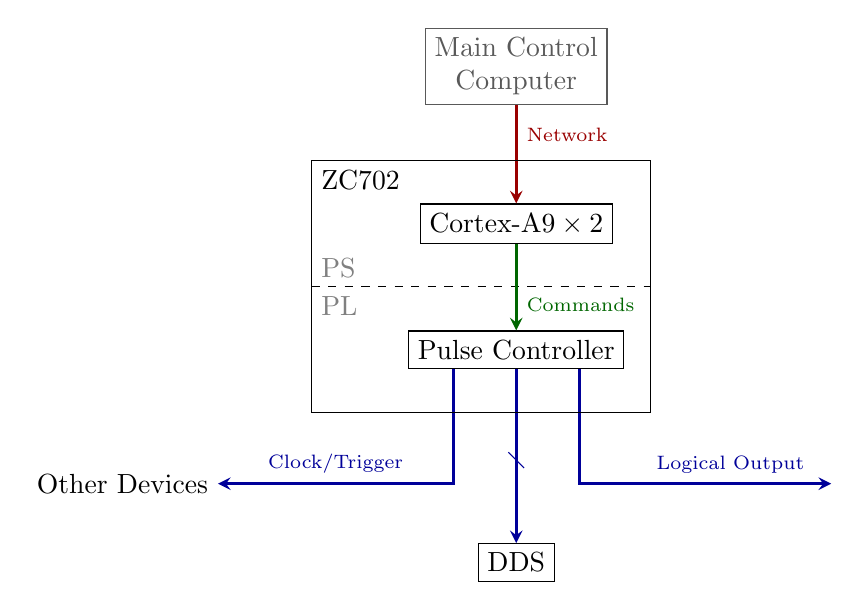
\begin{tikzpicture}
  \node[draw,align=center,gray!70!black] at (0, 2.8) (Computer) {Main Control\\Computer};
  \node[draw] at (0, 0.8) (CPU) {$\text{Cortex-A9}\times2$};
  \node[draw] at (0, -0.8) (FPGA) {Pulse Controller};
  \node at (-5, -2.5) (External) {Other Devices};
  \node[draw] at (0, -3.5) (DDS) {DDS};

  \draw[->,>=stealth,line width=1,red!60!black]
  (Computer.south) -- node[right,pos=0.3] {\scriptsize Network} (CPU.north);
  \draw[->,>=stealth,line width=1,blue!60!black] ([xshift=-0.8cm] FPGA.south) |-
  node[above,pos=0.75] {\scriptsize Clock/Trigger} (External.east);
  \draw[->,>=stealth,line width=1,blue!60!black] (FPGA.south) -- (DDS.north);
  \draw[blue!60!black] (-0.1, -2.1) -- (0.1, -2.3);
  \draw[->,>=stealth,line width=1,blue!60!black] ([xshift=0.8cm] FPGA.south) |-
  node[above,pos=0.8] {\scriptsize Logical Output} (4, -2.5);

  \draw (-2.6, -1.6) rectangle (1.7, 1.6);
  \draw[dashed] (-2.6, 0) -- (1.7, 0);
  \node[above right,gray] at (-2.6, 0) {PS};
  \node[below right,gray] at (-2.6, 0) {PL};
  \node[below right] at (-2.6, 1.6) {ZC702};
  \draw[->,>=stealth,line width=1,green!40!black]
  (CPU.south) -- node[below right] {\scriptsize Commands} (FPGA.north);
\end{tikzpicture}

\end{document}
